% This is a template for Ph.D. dissertations in the UCI format.

% All fonts, including those for sub- and superscripts, must be 10 points or larger.
% Recommended sizes are 14-point for chapter headings, 12-point for the main body of text
% and figure/table titles, and 10-point for footnotes, sub- and super-scripts, and text in
% figures and tables.
\documentclass[12pt,fleqn]{ucithesis}

\usepackage{amsmath}
\usepackage{array}
\usepackage{bm}
\usepackage{boxedminipage}
\usepackage{graphicx}
\usepackage{natbib}
\usepackage{path}
\usepackage{psfrag}
\usepackage{relsize}
\usepackage{subfigure}

\usepackage{url} 
\usepackage{todonotes}
\usepackage{alltt}
\usepackage{comment}
\usepackage{booktabs}
\usepackage{multirow}
\usepackage{listings}
\usepackage{multicol}

\usepackage{tikz}
\usetikzlibrary{decorations.pathreplacing,calc}
\newcommand{\tikzmark}[1]{\tikz[overlay,remember picture] \coordinate (#1);}

% plainpages=false fixes the "duplicate ignored" error with page counters
% Set pdfborder to 0 0 0 to disable colored borders around PDF hyperlinks
\usepackage[plainpages=false,pdfborder={0 0 0}]{hyperref}

% Uncomment the following line to enable Unicode support. This will allow you
% to enter non-ASCII characters (such as accented characters) directly without
% having to use LaTeX's awkward escape syntax (e.g., \'{e})
% NOTE: You may have to install the ucs.sty package for this to work. See:
% http://www.unruh.de/DniQ/latex/unicode/
% \usepackage[utf8x]{inputenc}

\newcommand{\term}{\emph}
\newcommand{\code}{\texttt}

\begin{document}

\thesistitle
{
	Information Flow for Dynamically Typed Languages:\\
	A Case Study of JavaScript
}

\degreename{Doctor of Philosophy}

% Use the wording given in the official list of degrees awarded by UCI:
% http://www.rgs.uci.edu/grad/academic/degrees_offered.htm
\degreefield{Information and Computer Science}

% Your name as it appears on official UCI records.
\authorname{Eric Hennigan}

% Use the full name of each committee member.
\committeechair{Professor First Last}
\othercommitteemembers
{
	Professor First Last\\
	Professor First Last
}

\degreeyear{2013}

\copyrightdeclaration
{
	{\copyright} {\Degreeyear} \Authorname
}

% If you have previously published parts of your manuscript, you must list the
% copyright holders; see Section 3.2 of the UCI Thesis and Dissertation Manual.
% Otherwise, this section may be omitted.
% \prepublishedcopyrightdeclaration
% {
% 	Chapter 4 {\copyright} 2003 Springer-Verlag \\
% 	Portion of Chapter 5 {\copyright} 1999 John Wiley \& Sons, Inc. \\
% 	All other materials {\copyright} {\Degreeyear} \Authorname
% }

% The dedication page is optional.
\dedications
{
	To my parents...
}

\acknowledgments
{
	I would like to thank...

	You must acknowledge grants and other funding assistance. 

	You may also acknowledge the contributions of professors and friends. 
	
	You also need to acknowledge any publishers of your previous work who have given you permission to incorporate that work into your dissertation. See Section 3.2 of the UCI Thesis and Dissertation Manual.
}

% Include, at minimum, a listing of your degrees and educational achievements with dates and the school where the degrees were earned. Also include the degree currently being attained.
\curriculumvitae
{
	% The following is a sample CV to get you started. Feel free to change it however you wish; there are no specific requirements regarding the formatting of your CV.

	\textbf{EDUCATION}

	\begin{tabular*}{1\textwidth}{@{\extracolsep{\fill}}lr}
		\textbf{Doctor of Philosophy in Computer Engineering} & \textbf{2008} \\
		\vspace{6pt}
		University of California, Irvine & \emph{Irvine, California} \\
		\textbf{Master of Science in Computer Engineering} & \textbf{2005} \\
		\vspace{6pt}
		University of California, Irvine & \emph{Irvine, California} \\
		\textbf{Bachelor of Science in Computer Engineering} & \textbf{1998} \\
		\vspace{6pt}
		Washington University & \emph{Saint Louis, Missouri} \\
		\textbf{Associate of Arts in Liberal Arts} & \textbf{1995} \\
		Johnson County Community College & \emph{Overland Park, Kansas} \\
	\end{tabular*}

	\vspace{12pt}
	\textbf{RESEARCH EXPERIENCE}

	\begin{tabular*}{1\textwidth}{@{\extracolsep{\fill}}lr}
		\textbf{Graduate Research Assistant} & \textbf{2003--2005} \\
		\vspace{6pt}
		University of California, Irvine & \emph{Irvine, California} \\
		\textbf{Research Assistant} & \textbf{1998--1999} \\
		Institute for Biomedical Computing & \emph{Saint Louis, Missouri} \\
	\end{tabular*}

	\vspace{12pt}
	\textbf{TEACHING EXPERIENCE}

	\begin{tabular*}{1\textwidth}{@{\extracolsep{\fill}}lr}
		\textbf{Teacher Trainee} & \textbf{2005--2006} \\
		\vspace{6pt}
		California Community College Internship Program & \emph{Santa Ana, California} \\
		\textbf{English Teacher} & \textbf{2001--2002} \\
		\vspace{6pt}
		Nova Group & \emph{Tarumi, Japan} \\
		\textbf{Math and Physics Teacher} & \textbf{1999--2001} \\
		Peace Corps & \emph{Tumu, Ghana} \\
	\end{tabular*}

	\vspace{12pt}
	\textbf{SELECTED HONORS AND AWARDS}

	\begin{tabular*}{1\textwidth}{@{\extracolsep{\fill}}lr}
		\textbf{Graduate Research Fellowship} & \textbf{2005--2008} \\
		\vspace{6pt}
		National Science Foundation & \\
		\textbf{Engineers' Class of 1991 Scholarship} & \textbf{1995--1998} \\
		\vspace{6pt}
		Washington University & \\
	\end{tabular*}

	\pagebreak

	\textbf{REFEREED JOURNAL PUBLICATIONS}

	\begin{tabular*}{1\textwidth}{@{\extracolsep{\fill}}p{4.5in}r}
		\textbf{Design, implementation, and test of a wireless peer-to-peer network for roadway incident exchange} & \textbf{2007} \\
		\multicolumn{2}{@{\extracolsep{\fill}}l}{International Journal of Vehicle Information and Communication Systems} \\
	\end{tabular*}

	\vspace{12pt}
	\textbf{REFEREED CONFERENCE PUBLICATIONS}

	\begin{tabular*}{1\textwidth}{@{\extracolsep{\fill}}p{4.75in}r}
		\textbf{Interactive Back-annotation of Worst-case Execution Time Analysis for Java Microprocessors} & \textbf{Aug. 2007} \\
		\multicolumn{2}{@{\extracolsep{\fill}}l}{Embedded and Real-Time Computing Systems and Applications} \vspace{6pt} \\
		\textbf{Identification and Removal of Program Slice Criteria for Code Size Reduction in Embedded Systems} & \textbf{May 2007} \\
		\multicolumn{2}{@{\extracolsep{\fill}}l}{International Embedded Systems Symposium} \vspace{6pt} \\
		\textbf{Toward a Unified Standard for Worst-Case Execution Time Annotations in Real-Time Java} & \textbf{Mar 2007} \\
		\multicolumn{2}{@{\extracolsep{\fill}}l}{Parallel and Distributed Real-Time Systems} \vspace{6pt} \\
		\textbf{A Survey of Worst-Case Execution Time Analysis for Real-Time Java} & \textbf{Mar 2007} \\
		\multicolumn{2}{@{\extracolsep{\fill}}l}{Java and Components for Parallelism, Distribution and Concurrency} \vspace{6pt} \\
		\textbf{Automatic Performance Visualization of Distributed Real-Time Systems} & \textbf{Apr. 2006} \\
		\multicolumn{2}{@{\extracolsep{\fill}}l}{Object-Oriented Real-Time Distributed Computing} \vspace{6pt} \\
		\textbf{RTZen: Highly Predictable, Real-time Java Middleware for Distributed and Embedded Systems} & \textbf{Nov. 2005} \\
		\multicolumn{2}{@{\extracolsep{\fill}}l}{Middleware} \vspace{6pt} \\
		\textbf{VADRE: A Visual Approach to Performance Analysis of Distributed, Real-time Systems} & \textbf{Jun. 2005} \\
		\multicolumn{2}{@{\extracolsep{\fill}}l}{Modeling, Simulation and Visualization Methods} \vspace{6pt} \\
		\textbf{Late Demarshalling: A Technique for Efficient Multi-language Middleware for Embedded Systems} & \textbf{Oct. 2004} \\
		\multicolumn{2}{@{\extracolsep{\fill}}l}{Distributed Objects and Applications} \vspace{6pt} \\
		\textbf{Adaptive Techniques for Minimizing Middleware Memory Footprint for Distributed, Real-Time, Embedded Systems} & \textbf{Oct. 2003} \\
		\multicolumn{2}{@{\extracolsep{\fill}}l}{Computer Communications} \\
	\end{tabular*}

	\vspace{12pt}
	\textbf{BOOKS}

	\begin{tabular*}{1\textwidth}{@{\extracolsep{\fill}}p{4.5in}r}
		\textbf{Web Developer's Guide To Visual J++ And ActiveX} & \textbf{1996} \\
		\multicolumn{2}{@{\extracolsep{\fill}}l}{Coriolis Group Books} \\
	\end{tabular*}

	\vspace{12pt}
	\textbf{SELECTED TECHNICAL PUBLICATIONS}

	\begin{tabular*}{1\textwidth}{@{\extracolsep{\fill}}p{4.75in}r}
		\textbf{CORBA is dead! Long live CORBA!} & \textbf{Mar. 2004} \\
		\multicolumn{2}{@{\extracolsep{\fill}}l}{Linux Magazine} \vspace{6pt} \\
		\textbf{Portability and the ARM Processor} & \textbf{Sep. 2003} \\
		\multicolumn{2}{@{\extracolsep{\fill}}l}{Dr. Dobb's Journal} \vspace{6pt} \\
		\textbf{Linux and the iPAQ, Arm in Arm} & \textbf{May 2003} \\
		\multicolumn{2}{@{\extracolsep{\fill}}l}{The C/C++ Users Journal} \\
	\end{tabular*}

	\vspace{12pt}
	\textbf{SOFTWARE}

	\begin{tabular*}{1\textwidth}{@{\extracolsep{\fill}}lr}
		\textbf{Volta} & \url{volta.sourceforge.net} \\
		\multicolumn{2}{@{\extracolsep{\fill}}l}{\emph{Development tools for distributed, hard real-time Java software}} \vspace{6pt} \\
		\textbf{Propelant} & \url{propelant.sourceforge.net} \\
		\multicolumn{2}{@{\extracolsep{\fill}}l}{\emph{Build automation of Linux for embedded systems}} \vspace{6pt} \\
		\textbf{HR-XSL} & \url{hr-xsl.sourceforge.net} \\
		\multicolumn{2}{@{\extracolsep{\fill}}l}{\emph{XML transformations for a curriculum vitae or résumé}} \\
	\end{tabular*}

	\vspace{12pt}
	\textbf{INVITED TALKS}

	\begin{tabular*}{1\textwidth}{@{\extracolsep{\fill}}lr}
		\textbf{Real-time Java} & \textbf{Feb. 2007} \\
		\vspace{6pt}
		Orange County Embedded Java Users' Group & \emph{Huntington Beach, California} \\
		\textbf{Static Timing Analysis for Multi-Robot Systems} & \textbf{Nov. 2006} \\
		Space and Naval Warfare Systems Center & \emph{San Diego, California} \\
	\end{tabular*}

	\vspace{12pt}
	\textbf{PROFESSIONAL MEMBERSHIPS}

	Institute of Electrical and Electronics Engineers (IEEE)
}

\thesisabstract
{
	The text of the abstract begins here. The text may contain a maximum of 350 words. Include a short statement of the 
problem you studied, a brief exposition of the methods and procedures employed in gathering the data, and a summary of your 
findings. No graphs, charts, or tables may be included.
}

\preliminarypages


\chapter{Motivation}

Many industrial and commercial institutions employ dynamically typed languages in systems which process sensitive information.
Programmers often find the high-level nature of these languages convenient for rapidly developing prototypes that meet the business need for quick deployment.
For example, Web applications have de facto standardized on JavaScript for client-side logic, which includes secure authentication.
In spite of the increasing demand for secure processing and communications, the semantics of dynamically typed languages, such as JavaScript, interferes static analysis techniques which could be used to verify application security~\cite{static-typing}.

In today's architecture, the web server delivers HTML and JavaScript to the client as an untyped string.
Web~2.0 applications contain server-side processing that injects user generated content and syndicated advertisements into pages assembled on demand.
Popular code frameworks which perform this composition are not themselves statically typed (as in the case of PHP, Ruby on Rails, Django).
The practice of including foreign content as an unsafe string provides attackers the opportunity to inject malicious code into a web page, in an attack known as Cross-Site Scripting (XSS).
The prevalence, persistence, scope, and danger~\cite{whitehat, mitre} of such attacks has given XSS the infamous moniker: ``buffer overflow of the web.''

\section{The Threat of Code Injection}

The most pernicious type of XSS attack allows the injected script to persist between browsing sessions, by residing in a server-side data store.
The canonical example of a \term{persistent} XSS attack involves a message board or web forum that allows the posting of user-generated content.
The site stores this content in a server-side database, so that it may be retrieved for viewing by other visitors.
When a malicious user bypasses textual filters and injects JavaScript into a forum posting, the site saves the script and inserts it into all pages that contain the post.
To become a victim, an innocent user needs only to view a page with the malicious post.

Many of the victims viewing the forum are simultaneously logged in to other more sensitive services (such as email, shopping, banking or brokerage accounts).
For most users, the web browser stores more personally identifying information about individual habits and interests than any other single application.
Additionally, web browsers also conveniently store login credentials for banking sites, webmail services, and many shopping sites, as well as form information containing your real name, address, phone number, and credit card numbers.
The potential for harvesting of sensitive user credentials via a forum post with malicious JavaScript presents a serious threat.

\section{Difficulties of Filtering User Input}

Currently, the most promoted mechanism for preventing script injection attacks is to filter out HTML and JavaScript code from user input.
Though user input filtering forms the first line of security defense of any website, not every malicious script can be deterministically identified.
Web frameworks which lack strong static typing further compound the problem because they cannot provably verify that all strings pass through a filter function before placement into the resulting page.

\subsection{HTML Identification}
\label{subsec:html-encoding}

The Web is constructed from various interrelated technologies: URLs for resource requests, HTML for page layout, CSS for content layout, JavaScript for page code, the JavaScript Object Notation (JSON) for object description, XML for data description, etc.
Each of these technologies has its own specification and set of allowed characters.
So many different character encodings exist that developers find it very difficult to track in what context a user-supplied string might appear on a page and how a browser interpret the string in that context.

These many different encodings allow an attacker to formulate strings that are acceptable in one context, but nefarious in another.
For example, characters such as `\texttt{<}', which has special meaning in the HTML specification, can be escaped in many different ways (see Table~\ref{tab:html-encoding}).
Historic design philosophies such as `being liberal in what you accept from others'~\cite{rfc761}, have coerced browsers into allowing whitespace (\texttt{<scr ipt>}) or mixed-case (\texttt{<ScrIpT>}) when matching HTML tags.
The acceptance of tags formatted in unconventional manners further contributes to the difficulty of identifying potentially malicious inputs.

\begin{table}[ht]
\centering
\begin{tabular}{l|ccccc}
 \textbf{Encoding Type} & \multicolumn{4}{c}{\textbf{Encoded variant of `\texttt{<}'}} \\
 \hline
 URL Encoding           & \texttt{\%3C} &&&\\
 HTML Entity            & \texttt{\&lt;} & \texttt{\&lt} & \texttt{\&LT;} & \texttt{\&LT} \\
 Decimal Encoding       & \texttt{\&\#60;} & \texttt{\&\#060;} & \texttt{\&\#0060;} & \texttt{\ldots} \\
 Hex Encoding           & \texttt{\&\#x3c;} & \texttt{\&\#x03c;} & \texttt{\&\#X3c} & \texttt{\ldots} \\
 Unicode                & \texttt{\textbackslash u003c} &&&\\
\end{tabular}
\caption{Examples of Character Encoding~\cite{secubat}.}
\label{tab:html-encoding}
\end{table}

\subsection{Script Identification}

Examples from RSnake's XSS Cheat Sheet~\cite{xsscheatsheet}\footnote{The XSS Cheat Sheet also provides a handy reference of malicious scripts that can be used to test user input filters} exhibit many ways in which a script can be encoded to bypass user input filters.
As a second line of defence, a web page can employ syntax filters and program analysis to restrict the running of malicious scripts~\cite{browsershield, corescript, webssari}.

Just as HTML has many different character encodings, JavaScript provides several syntaxes for accessing an object's properties.
For example, each of the following three lines create a dialog box with the contents of a page's cookie:

\begin{alltt}
alert(document.cookie)
alert(document['cookie'])
with(document) alert(cookie)
\end{alltt}

This multiplicity interferes with routines that attempt to identify malicious code when filtering user input.
To provide a clear demonstration of difficulties encountered by input filtering, Hasegawa~\cite{xssfilters} manufactured the following JavaScript snippet that calls \texttt{alert(1)}, yet contains no alphanumeric characters:

\begin{alltt}
($=[$=[]][(__=!$+$)[_=-~-~-~$]+({}+$)[_/_]+($$=($_=!''+$)
[_/_]+$_[+$])])()[__[_/_]+__[_+~$]+$_[_]+$$](_/_)
\end{alltt}

\section{The Last Line of Defence}

This work assumes that the web application's filter defenses are incomplete and non-exhaustive.
The attacker is able to bypass the filters and store malicious JavaScript in the web site's database.
The server code responsible for assembling pages trusts the database content and includes the code in pages viewable by innocent users of the application.

\begin{comment}
The persistent XSS attack just given illustrates two fundamental principals of web security: (1) user generated content cannot be trusted, and (2) data stored on your own servers should not necessarily be trusted.

The second principal is most concerning, and the one we wish to combat.
Within the browser, the execution semantics of JavaScript,
\end{comment}

Persistent XSS attacks have in the past shut down popular internet services.
For example, in 2005, the `Samy' worm~\cite{samy} set a world record for viral spreading and forced MySpace to suspend service in order to purge the work from their database.
In 2007, the RightMedia Trojan propagated itself via malicious banner advertisements delivered through a trusted syndication network.
These ads appeared on popular sites such as Yahoo! Photobucket and MySpace.
In 2007, Nduja~\cite{nduja} authored a ``Cross Webmail Worm'' that was able to propagate itself across four webmail providers among the most popular in Italy.
On each of the four webmail providers separate functionality for both infection and propagation needed to be developed, making this worm the first to spread across different web applications.
Though dated, these examples are notable not only for setting records, but also for demonstrating the relative ease with which a clever user can control the actions taken by millions of other browsers.
The architectural problems underlying these attacks have not been solved.

\subsection{Preventing Malicious Action}

\begin{comment}
\todo{categorize XSS?}

\begin{itemize}
    \item say that js handles sensitive info
    \item delineate injection
    \item categorize xss
    \item pound-include problem
    \item scare-monger prevalence as `buffer overflow'
    \item sandbox + same origin policy
    \item have to setup an attacker model?
\end{itemize}

\end{comment}

Rather than rely entirely on filtration that attempts to identify and reject attacker supplied code, this work allows the malicious code to execute under new semantics which track the information dependence of runtime values.
We assume that without generating external signals (network traffic) the execution of code within the browser sandbox results in no harm.
This work implements FlowCore, interpreter-level information flow framework written for WebKit's JavaScriptCore virtual machine.

FlowCore introduces a general set of information flow bytecodes (Section~\ref{sec:bytecodes}) applicable to any interpreter for a dynamically typed language.
The bytecodes provide runtime instructions for manipulating information flow data structures (Section~\ref{sec:f-stack}) for each of the control flow structures (Section~\ref{sec:control-flow}) in the JavaScript language.
Additionally, the VM tags every JavaScript value with a label (Section~\ref{sec:tagging}) that records the principals which have influenced the value.
A network monitor within the web browser prevents malicious program behavior at runtime by enforcing a policy shipped with the web page (Section~\ref{sec:policy}).

\begin{comment}
on using information flow techniques which can detect and prevent malicious behavior of executing programs.

- change language semantics
- augment memory model with labels
- detect and intercept xss
- prevent information leakage

Combine earlier approaches into a universal and comprehensive framework
- decentralized labeling
- support more flexible policies
- hybrid static/dynamic analysis
- dynamically track information flow
- pervasively works at the lowest layer
\end{comment}


\chapter{Related Work}
\todo{There are two outstanding problems: 1. label creep, 2. can't track passive indirect flows.}
\chapter{Flow Terminology}

\label{sec:terminology}

\begin{comment}
\begin{table*}
\centering
\begin{tabular}{ccccm{2.5cm}}
\toprule
Category & Descriptor & Example & Flow & Required Analysis \\
\midrule[\heavyrulewidth]
\multirow{3}{*}{Explicit} & Direct &
\begin{js-embed}
b = a
\end{js-embed} & a $\rightarrow$ b & Dataflow\\
\cmidrule(r){2-5} & Indirect &
\begin{js-embed}
b = foo(_, a, _)
c = bar(_, b, _)
\end{js-embed}
& a $\rightarrow$ c & Dataflow (transitive) \\
\hline
\multirow{7}{*}{Implicit} & Active &
\begin{js-embed}
a = true
b = 0
if (a)
   b = 1
else
   ...
\end{js-embed}
& a $\rightarrow$ b & Control Flow (dynamic)\\
\cmidrule(r){2-5} & Passive &
\begin{js-embed}
a = true
c = 0
if (a)
   ...
else
   c = 1
\end{js-embed}
& a $\rightarrow$ c & Control Flow (static)\\
\bottomrule
\end{tabular}
\caption{Terminology of Information Flows.}
\label{table:terminology}
\end{table*}
\end{comment}

After the founding of information flow as a program analysis technique in the late 1970's by Denning and Denning~\cite{denning.denning+77}, the field lay relatively quiescent until recently.
Since the mid 2000's, because of enhancements in the interactivity of web pages and the steady rise in online commerce, there has been a fervent and earnest push for greater data security in web browsers and web applications.
Because these programs use dynamically typed languages they cannot use a static type checker to prove and enforce program properties.
Lacking a mechanism for verifying security and data handling properties, information flow remains the most promising approach for detecting and preventing information leakage in web applications.

The rapid creation of so many new systems~\cite{chugh.etal+09, yaowen.etal+04, jang.etal+10, robertson.vigna+09, vogt.etal+07} using information flow techniques to attack web security problems has led to a difficulty in comparing research results across implementations.
For example, some authors implement simple data tainting while others use wrapper objects or dynamic rewriting techniques.
I find disconcerting the lack of a terminology for describing, in detail, exactly which categories of information flow a system can detect.
Of more critical importance, without adequate vocabulary, my literature review finds researchers somewhat negligent in expressing the limits of their system's capabilities.
As a result, the boundary line circumscribing the state of the art remains painfully fuzzy.

Recent work applying information flow techniques has overloaded terminology established by Denning and Denning~\cite{denning.denning+77}.
For example, when Jang~et~al.~\cite{jang.etal+10} describe the capabilities of their JavaScript rewriting system, they introduce the term ``indirect'' to describe a flow for which they found no previous research.
This ``new'' terminology unfortunately overloads an existing use of the term by Denning and Denning~\cite{denning.denning+77}, prompting the creation of this chapter.

This work bases itself on Denning and Denning's~\cite{denning.denning+77} original categorization of the types of flows which can occur in an executable program because this categorization has become standard in the field.
However, since their categorization lacks sufficient precision for more modern implementations, especially in application to dynamically typed languages, this work also introduces a refinement of the standard terminology.
This work offers more precise and descriptive designations of the established types of information flows in the most compatible manner possible.
For each flow identified, this work also illustrates the language mechanisms responsible for the information flow.
Finally, I demonstrate the descriptive utility of the new terminology by mapping each flow to the program analysis required to detect it.

This chapter refines the two categories of information flow established by Denning and Denning~\cite{denning.denning+77}, explicit flows (Section~\ref{sec:explicit-flow}) and implicit flows (Section~\ref{sec:implicit-flow}).

\section{Explicit Information Flows}
\label{sec:explicit-flow}

Explicit information flows occur as a result of data flow dependence.
This dependence can be either \emph{direct} or \emph{indirect} (see Table~\ref{table:explicitterminology}).
Denning and Denning~\cite{denning.denning+77} establish both the definition of explicit information flows and the descriptors shown in Table~\ref{table:explicitterminology}.

\begin{table*}[h]
\centering
\begin{tabular}{ccccm{2.5cm}}
\toprule
Category & Descriptor & Example & Flow & Required Analysis \\
\midrule[\heavyrulewidth]
\multirow{3}{*}{Explicit} & Direct &
\begin{js-embed}
b = a
\end{js-embed}
& a $\rightarrow$ b & Dataflow\\
\cmidrule(r){2-5} & Indirect &
\begin{js-embed}
b = foo(_, a, _)
c = bar(_, b, _)
\end{js-embed}
& a $\rightarrow$ c & Dataflow (transitive) \\
\bottomrule
\end{tabular}
\caption{Terminology of Explicit Information Flows.}
\label{table:explicitterminology}
\end{table*}

\begin{description}
\item{
\textbf{Direct Explicit Flows} occur when a value is influenced as a result of direct data transfer, such as an assignment.
A simple single-statement intra-procedural dataflow analysis can identify these flows.
Table~\ref{table:explicitterminology} illustrates an intuitively clear example of this type of flow which occurs in the code sample: \texttt{var pub = secret}.
Subexpressions involving more than one argument also have a direct explicit information flow from all argument values to the operator's resulting value.
Any labeling or tagging mechanism which propagates the security type information across direct explicit flows includes basic rules for each of the language's operators.
}

\item{
\textbf{Indirect Explicit Flows} occur as the transitive closure of direct flows.
Identification of indirect flows requires more powerful multi-statement or inter-procedural dataflow analysis.
The code example for indirect flows in Table~\ref{table:explicitterminology} shows their transitive nature via a functional dependence.
This paper preserves the use of the term ``indirect'' as originally defined by Denning and Denning~\cite{denning.denning+77} and not as overloaded by Jang~et~al.~\cite{jang.etal+10}.
}
\end{description}

\section{Implicit Information Flows}
\label{sec:implicit-flow}

Implicit information flows occur when a value is influenced as a result of control flow dependence.
This dependence can be either \term{active}, corresponding to a runtime dependence, or \term{passive}, corresponding to a static dependence.
Although Denning and Denning~\cite{denning.denning+77} establish the term \term{implicit flow} they did not refine the category into these two descriptors.

\begin{table*}[h]
\centering
\begin{tabular}{ccccm{2.5cm}}
\toprule
Category & Descriptor & Example & Flow & Required Analysis \\
\midrule[\heavyrulewidth]
\multirow{7}{*}{Implicit} & Active &
\begin{js-embed}
a = true
b = 0
if (a)
   b = 1
else
   ...
\end{js-embed}
& a $\rightarrow$ b & Control Flow (dynamic)\\
\cmidrule(r){2-5} & Passive &
\begin{js-embed}
a = true
c = 0
if (a)
   ...
else
   c = 1
\end{js-embed}
& a $\rightarrow$ c & Control Flow (static)\\
\bottomrule
\end{tabular}
\caption{Terminology of Implicit Information Flows.}
\label{table:implicitterminology}
\end{table*}

\begin{description}
\item{
\textbf{Active Implicit Flows} occur when a value depends depends on a previously taken control flow branch \term{at runtime}.
Identification of this dependence requires a tracked program counter and a recorded history of control flow branches taken during program execution.
Presently, systems which track the program counter in order to propagate dependence information are known as ``dynamic information flow tracking'' systems.
Because the literature lacks a refined terminology for the two descriptors of implicit flow, Jang~et~al.~\cite{jang.etal+10} coin the term ``indirect flow'' to refer to this kind of flow.
}

\item{
\textbf{Passive Implicit Flows} occur when a value depends on a control flow branch \emph{not taken} during program execution.
Identification of this dependence requires a static analysis prior to program execution.
Because the dependence follows code paths not taken at runtime, these flows are notoriously difficult to detect in dynamic programming languages.
Unfortunately, even static languages include features, such as object polymorphism and reference returning functions, which make the destination of an assignment unknown at compile time.
Dynamic programming languages, such as JavaScript, include runtime field lookup, prototype chains, and the ability to load additional code at runtime via \texttt{eval}.
These features prohibit even runtime analysis from identifying all the values possibly influenced in all alternative control flow branches.
}

\end{description}

\section{The Tracking Capabilities of \FlowCore}
\label{sec:tracking-capabilities}

%Previous work attempts to secure active information flows using through staged analysis~\cite{staged-javascript} and lightweight static analysis~\cite{XSS-tainting}.
\FlowCore\ modifies the JavaScript VM to track both direct and indirect explicit flows at runtime.
The transitive dataflow analysis include the tracking of values passed to and returned from function calls.
\FlowCore\ also implements a runtime data structure for recording the history of the program counter (see~\ref{sec:control-flow-stack}) which allows the tracking of implicit active flows.
Because of the onerous analysis required, \FlowCore\ makes no attempt to track influence via passive control flow.
Instead, this system focuses exclusively on complete runtime tracking of implicit active flows, for all of JavaScript's control structures (see~\ref{sec:feature-catalog}).


\chapter{Label System Design Considerations}

Designing the labeling system supporting information flow tracking took special consideration.
FlowCore could have been written using one of two possible implementations of security types (Section~\ref{sec:implementation}): (1) extending of the tagged pointer representation and (2) introducing a security wrapper object.
Before choosing one implementation over the other, we first examine how each option affects the labeling of primitive values and interned objects and how the labeling mechanism will impact memory requirements and the garbage collector (Section~\ref{sec:analysis}).
We corroborate this analysis with a report on our experience during implementation (Section~\ref{sec:experience}).
Finally, we show how this work compares with that of others (Section~\ref{sec:related-work}), and finish with a recommendation that an extension of the tagged pointer representation meets the requirements of a dynamic information flow security type system and has the least implementation effort (Section~\ref{sec:conclusion}).

\section{Possible Implementations}
\label{sec:implementation}

Before discussing the details of the two possible implementations of dynamic security types, we first give a review of the existing dynamic type system that WebKit's JavaScriptCore VM employs.

\subsection{Existing Type System}

Many implementations of dynamically typed languages follow a common approach of using a tagged union to represent each possible primitive or object reference type~\cite{gudeman1993representing}.
In JavaScriptCore, this union takes the form of a 64-bit word, within the class \code{JSValue}.
Figure~\ref{fig:base-encoding} illustrates the union's fields as ordered on a big-endian\footnote{On a little-endian machine the order of the \code{tag} and \code{payload} fields are swapped.}, 64-bit machine.

Within a \code{JSValue}, a leading value of \texttt{0xFFFF} distinguishes 32-bit JavaScript integers.
Doubles are offset (under bitwise integer interpretation) by the value $2^{48}$ to ensure that all values have at least a leading value of \texttt{0x0001}.
JavaScriptCore maintains a garbage collected heap which stores JavaScript objects with 64-bit alignment.
Pointers to garbage collected JavaScript objects all begin with a leading \texttt{0x0000}, which nominally reduces the address space to 48 bits\footnote{Modern 64-bit processors only supply 48 bits of addressable space, so JavaScriptCore's chosen pointer encoding does not reduce the actual usable space.}.
The special JavaScript values \code{null}, \code{false}, \code{true}, and \code{undefined} each have bit 1 set, to distinguish them from properly aligned pointer values.
JavaScriptCore also encodes two additional values, again at invalid pointer addresses, which are not defined within the JavaScript language: \code{empty}, which represents array holes and uninitialized \code{JSValue}s, and \code{deleted}, which is used in hash table code.

\begin{comment}
   1  2   3      4
 0123456789abcdef
 0xffff ffff ffff ffff
    16   32        64

 signal nan:
 0x7ff0 0000 0000 0001 to
 0x7ff7 ffff ffff ffff
 or
 0xfff0 0000 0000 0001
 0xfff7 ffff ffff ffff

 quiet nan:
 0x7ff8 0000 0000 0001
 0x7fff ffff ffff ffff
 or
 0xfff8 0000 0000 0001
 0xffff ffff ffff ffff

 1 111 1 111 1 111 1---
 F     F     F     >8 

 E = 15 - 1 = 14 = 8 + 4 + 2
                   0111
                    - 1 // convert to actual double
                   0110 = 13
                   6

                   jsNan = 7ff8 0000 0000 0000
                           ffff                  tag type number
                           ----
                           true

                    jsNan -> asDouble
                    7ff8 0000 0000 0000
                -      1 0000 0000 0000       double encode offset
                   ---------------------
                    7ff7 0000 0000 0000       // now a signaling nan

\end{comment}

\begin{figure}[h]
    \centering
\begin{tabular}{cc}
    \begin{minipage}[h]{.5\textwidth}
        \vfill
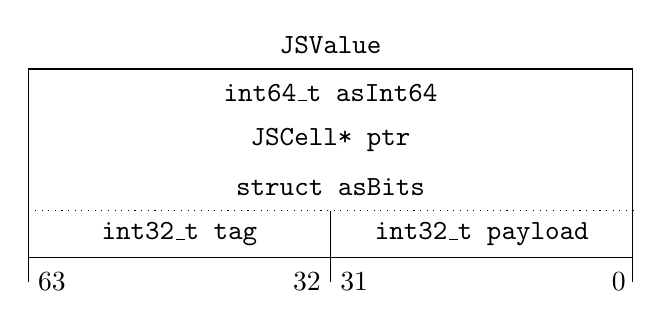
\begin{tikzpicture}[scale=.12]
 \draw[anchor=center] (32,2.5) node {\code{JSValue}};
 \draw (0,0) -- (0,-20) -- (64,-20) -- (64,0) -- cycle;
 \draw[anchor=center] (32,-2.5) node {\code{int64\_t asInt64}};
 %\draw[anchor=center] (32,-7.5) node {\code{double asDouble}};
 \draw[anchor=center] (32,-7.5) node {\code{JSCell* ptr}};
 %\draw (0,-10) -- (64,-10);
 \draw[anchor=center] (32,-12.5) node {\code{struct asBits}};
 \draw [dotted] (0,-15) -- (64,-15);
 \draw (32,-15) -- (32,-22.5);
 \draw[anchor=center] (16,-17.5) node {\code{int32\_t tag}};
 \draw[anchor=center] (48,-17.5) node {\code{int32\_t payload}};
 \draw (0,-20) -- (0,-22.5);
 \draw (64,-20) -- (64,-22.5);
 \node at (62.5,-22.5) {0};
 \node at (34.5,-22.5) {31};
 \node at (29.5,-22.5) {32};
 \node at (2.5,-22.5) {63};
\end{tikzpicture}
        \vfill
\end{minipage}
&
\begin{tabular}{c|l}
    bit values & type  \\
\hline
    \texttt{0000 0000 0000 0000} & \texttt{empty} \\
    \texttt{0000 0000 0000 0004} & \texttt{deleted} \\
    \texttt{0000 0000 0000 0002} & \texttt{null} \\
    \texttt{0000 0000 0000 0006} & \texttt{false} \\
    \texttt{0000 0000 0000 0007} & \texttt{true} \\
    \texttt{0000 0000 0000 000a} & \texttt{undefined} \\
    \texttt{0000 pppp pppp pppp} & \texttt{pointer} \\
    \texttt{0001 dddd dddd dddd} & \tikzmark{2nd} \multirow{3}{*}{\texttt{  double}} \\
    \texttt{\vdots} & \\
    \texttt{FFFE dddd dddd dddd} & \tikzmark{4th} \\
    \texttt{FFFF 0000 iiii iiii} & {integer}
\end{tabular}
\begin{tikzpicture}[overlay, remember picture]
    \draw [decoration={brace,amplitude=.5em}, decorate]
    ($(2nd)+(0,1ex)$) -- ($(4th)+(0,1ex)$);
\end{tikzpicture}

\end{tabular}
\caption{
    \label{fig:base-encoding}
    Representation of the internal \code{JSValue} class and the dynamic type encoding used in Webkit's JavaScriptCore VM.}
\end{figure}

\begin{comment}
         *     False:     0x06 =     4 + 2
         *     True:      0x07 =     4 + 2 + 1
         *     Undefined: 0x0a = 8     + 2
         *     Null:      0x02 =         2

         * These values have the following properties:
         * - Bit 1 (TagBitTypeOther) is set for all four values, allowing real pointers to be
         *   quickly distinguished from all immediate values, including these invalid pointers.
         * - With bit 3 is masked out (TagBitUndefined) Undefined and Null share the
         *   same value, allowing null & undefined to be quickly detected.
         *
         *     Deleted:   0x0
         *     Empty:   0x4
         * No valid JSValue will have the bit pattern 0x0, this is used to represent array
         * holes, and as a C++ 'no value' result (e.g. JSValue() has an internal value of 0).
        // These special values are never visible to JavaScript code; Empty is used to represent
        // Array holes, and for uninitialized JSValues. Deleted is used in hash table code.
        // These values would map to cell types in the JSValue encoding, but not valid GC cell
        // pointer should have either of these values (Empty is null, deleted is at an invalid
        // alignment for a GC cell, and in the zero page).
         */
\end{comment}

\subsection{Fat Value Technique}\label{sec:fat-values}
We can achieve dynamic information flow security by attaching, onto each runtime value, additional bits which encode a pointer, handle, or taint value representing the security type.
We term this technique the \term{fat value} approach, and extend the existing \code{JSValue} representation with an additional 64-bit word to hold the security type.
As shown in Figure~\ref{fig:fat-encoding}, each value within the interpreter then becomes 128-bits and contains both the originally encoded value and its security tag.

\begin{figure}[h]
\begin{minipage}[h]{.7\textwidth}
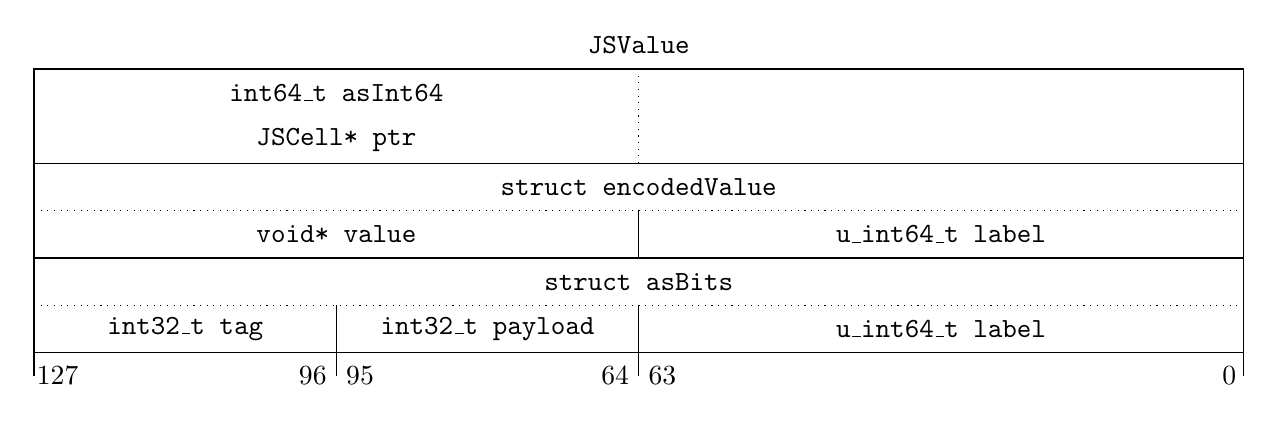
\begin{tikzpicture}[scale=.12]
 \begin{scope}[shift={(0,0)}]
 \draw (0,-5) rectangle (128,-15);
 \draw[anchor=center] (64,-2.5) node {\code{JSValue}};
 %\draw (64,-5) -- (64,-15);
 \draw[anchor=center] (32,-7.5) node {\code{int64\_t asInt64}};
 %\draw[anchor=center] (32,-12.5) node {\code{double asDouble}};
 \draw[anchor=center] (32,-12.5) node {\code{JSCell* ptr}};
 \draw[dotted] (64,-5) -- (64,-15);
 \end{scope}

 \begin{scope}[shift={(0,-15)}]
 \draw (0,0) rectangle (128,-10);
 \draw[dotted] (0,-5) -- (128,-5);
 \draw (64,-5) -- (64,-10);
 \draw[anchor=center] (64,-2.5) node {\code{struct encodedValue}};
 \draw[anchor=center] (32,-7.5) node {\code{void* value}};
 \draw[anchor=center] (96,-7.5) node {\code{u\_int64\_t label}};
 \end{scope}

 \begin{scope}[shift={(0,-25)}]
 \draw (0,0) rectangle (128,-10);
 \draw[anchor=center] (64,-2.5) node {\code{struct asBits}};
 \draw[dotted] (0,-5) -- (128,-5);
 \draw[anchor=center] (16,-7.5) node {\code{int32\_t tag}};
 \draw[anchor=center] (48,-7.5) node {\code{int32\_t payload}};
 \draw[anchor=center] (96,-7.5) node {\code{u\_int64\_t label}};
 \draw (32,-5) -- (32,-10);
 \draw (64,-5) -- (64,-10);
 \end{scope}

 \begin{scope}[shift={(0,-35)}]
 \draw (0,0) -- (0,-2.5);
 \node at (2.5,-2.5) {127};
 \node at (29.5,-2.5) {96};
 \draw (32,0) -- (32,-2.5);
 \node at (34.5,-2.5) {95};
 \node at (61.5,-2.5) {64};
 \draw (64,0) -- (64,-2.5);
 \node at (64+2.5,-2.5) {63};
 \node at (126.5,-2.5) {0};
 \draw (128,0) -- (128,-2.5);
 \end{scope}
\end{tikzpicture}
\end{minipage}
 \caption{Fat value encoding scheme.}
 \label{fig:fat-encoding}
\end{figure}\hfill

The fat value technique requires modifying the core representation of all values within the VM.
While performing this modification on an arbitrary dynamic language VM is not necessarily a trivial undertaking, the designers of JavaScriptCore have conveniently encapsulation the type inspection and conversion methods in the \code{JSValue} class.
This practice makes the modification easier than on other JavaScript VM's such as SpiderMonkey.
However, appropriately tagging each value with a security label still requires manual inspection of all code sites which create new values.
Additionally, doubling the size of the core datatype also doubles the memory space requirements of any running program: the VM allocates twice as much space for the same number of core values.

\subsection{Security Wrapper Technique}\label{sec:cloaks}

Another mechanism, known as the security wrapper technique, can also achieve the goal of attaching a security label to each value.
In this mechanism, the VM labels JavaScript objects by extending them with an additional internal field.
We introduce an internal security wrapper object which stores a primitive together with its label.
Throughout our analysis, we shall refer to this wrapper object as a \term{cloak} and any value held within the wrapper as a \term{cloaked} value.
Figure~\ref{fig:security-wrapper} provides a visualization of the cloak mechanism.

\begin{figure}[h]
 \centering
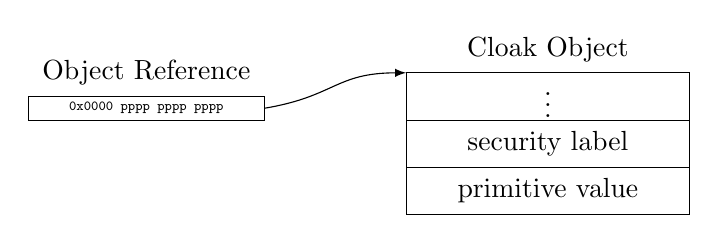
\begin{tikzpicture}[scale=.12]
    \node[anchor=center] at (12.5,2.5+2.5) {Object Reference};
    \node[anchor=center] at (12.5,2.5/2) {\tiny \texttt{0x0000 pppp pppp pppp}};
    \draw (0,0) rectangle (25,2.5);

    \coordinate (Obj) at (40,5);
    \node[anchor=center] at ($(Obj)+(15,2.5)$) {Cloak Object};
    \draw (Obj) rectangle ($(Obj)+(30,-15)$);
    \node[anchor=center] at ($(Obj)+(15,-2.5)$) {\vdots};
    \draw ($(Obj)-(0,5)$) -- ($(Obj)+(30,-5)$);
    \node[anchor=center] at ($(Obj)+(15,-5-2.5)$) {security label};
    \draw ($(Obj)-(0,10)$) -- ($(Obj)+(30,-10)$);
    \node[anchor=center] at ($(Obj)+(15,-10-2.5)$) {primitive value};

    \draw[-latex] (25,2.5/2) .. controls (25+15/2,2.5) and (25+15/2,5) ..  (Obj);

\end{tikzpicture}
\caption{Security wrapper scheme.}
\label{fig:security-wrapper}
\end{figure}

Internally, JavaScriptCore already supports wrapper classes for Strings and Dates, as well as automatic objection promotion for Numbers and Booleans.
Given this information, we might expect fewer modifications to be made to the underlying VM, as this change only requires the introduction of a new subclass of the existing \code{JSWrapperObject}.

However, implementing the wrapper class is not exactly trivial, even with the help of an existing framework.
From the perspective of the JavaScript program, a cloak object must mimic, in every circumstance, the same behavior as the primitive it cloaks.
Under no circumstances should the presence (or absence) of a security wrapper ever become evident to a JavaScript program, otherwise attacker provided code could exploit the difference in behavior.
%We make an exception to this guideline for policy violations, which have the side effect of halting the VM.
The wrapper must remain distinguishable to the VM, however, so that it can enforce information flow security.

Meeting this restriction is not presently possible using the existing wrapper framework.
The primary goals of the existing wrapper class is to collect those datatypes (Date, String, Number, and Boolean) which can be stored within the space of a \code{JSValue}.
As a result, the treatment of wrapped objects within the interpreter does not sufficiently take into account the behavioral differences between objects and primitives.
For example, in Listing~\ref{list:boolean}, a Boolean object wrapping the primitive value \code{false} behaves according to the rules governing objects rather than those of the primitive boolean value.
Consequently, the existing framework poses an imperfect fit for implementing information flow security, because it does not guarantee perfect transparency (from the perspective of a JavaScript program) when used to wrap primitives.

\begin{lstlisting}[caption={JavaScript considers objects as `truthy' values.},label={list:boolean}]
js> var x = new Boolean(false)
js> if (x) { print("x is true"); }
x is true
\end{lstlisting}

\section{Impacts on the Virtual Machine}
\label{sec:analysis}

Now that we have introduced two viable techniques for implementing information flow security, we analyze how each performs when labeling primitives, how each handles interned objects, and what impacts each has on the garbage collector.

\subsection{Labeling Primitives}\label{sec:primitives}

%Although the tagged pointer encoding is an implementation detail, this decision has had side effects which have leaked into the JavaScript specification.
%The foundational JavaScript VM, SpiderMonkey, initially implemented a tagged pointer encoding scheme for the 32-bit machines of that era.
%For example, SpiderMonkey's original 32-bit implementation used 1 bit for the integer type tag, and 31 bits for integer values.
%This design forced the language specification~\cite{ecma} to provide a coercion of any integer which cannot be represented by 31-bits to the \texttt{double} type.

The existing core datatype in JavaScriptCore uses a NaN encoding scheme that enables the value and type tag to coexist in the same memory structure.
The tagged pointer technique has the benefit of allowing the VM to perform operations on primitives quickly and directly.
Unfortunately, many common operators, such as \texttt{+}, behave differently depending on the types of the arguments.
Not only must the VM first inspect the type of the core values involved before dispatching the operation, but it then also unpacks the payload of the arguments from their encoding.

Using the fat value approach requires modifying the core value representation, extending it with additional bits to hold the security type.
This modification impacts the mechanisms used to encode and decode primitive values, as well as the type inspection routines.
JavaScriptCore uses an Object-Oriented design that encapsulates the type inspection logic, preventing it from dispersing across the VM implementation.
However, we must still manually audit each site at which the VM creates \code{JSValue}s so that the appropriate security label can be set.

Alternatively, the cloak approach requires the creation of a wrapper object for each labeled primitive.
Although the cloak easily holds both the core value representation of the primitive as well as the security type, the presence of a cloak object negatively impacts the runtime type inspection logic.
Where before the VM would previously inspect a primitive, it now dispatches inspection logic on a cloak object.
This extra layer of indirection severely degrades the performance of the very operations for which primitives are optimized.

The WebKit developers have designed JavaScriptCore as an embeddable interpreter.
Systems external to the JavaScript engine, such as the DOM framework of the WebKit browser, reflect their own classes into the JavaScriptCore engine.
This reflection occurs via a layer of interface classes\footnote{The WebKit build system automatically generates the interface classes.}, which each inherit a JavaScriptCore class such as \code{JSNonFinalObject}.
Should an external system expect certain fields to contain raw primitives (such as integers), it will fail when receiving a cloaked value.
When implementing the cloak scheme, we must either prohibit cloaks from escaping the JavascriptCore VM or modify the interface layer to automatically uncloak.
Both of these solutions leave the browser's external systems open as an information side channel.

To avoid observable semantic changes that could be exploited by an attacker, cloaks must also remain completely invisible to the JavaScript programmer.
For example, even though we implement cloaks as a native \code{JSObject} within the VM, we cannot allow a JavaScript program to set a property on a cloaked primitive.
Additionally, some JavaScript operators, such as \code{typeof}, require introducing an additional special case.
For example, a cloaked integer reports the type of the cloaked value, ``\code{number}'', rather than the type of the cloak, ``\code{object}''.
Should the VM use this operator internally for a type dispatch, it would then pass the value into a native routine expecting a raw primitive value.
To reduce the amount of implementation effort, we seek to avoid hunting down all the type dispatch sites and introducing these special cases.

When we compare the fat value approach to the cloak approach, an interesting semantic difference arises:
In the fat value approach, we attach the security type to the primitive value or object reference, as part of the tagged pointer encoding.
In the cloak approach, each object receives an internal field in store its security label while primitives are cloaked with an extra layer of indirection.

\todo{I haven’t fully explored the difference between having a labeled reference vs having a labeled object, but I think the difference is analogous to having an Access Control Listing by columns vs Object Capabilities by rows, as discussed in Capability Myths Demolished.}
% At this point I am in favor of the fat value approach, because I’m liking the reference semantics, and the transparency with which primitives can be labeled. I’m also willing to accept the cost of having fatter values.

\section{Implementation Experience}
\label{sec:experience}

\section{Related Implementations}
\label{sec:related-work}

\section{Chosen Implementation for FlowCore}
\label{sec:conclusion}

\chapter{Label Propagation}
\chapter{Bytecodes}
\chapter{JavaScript Feature Catalog}
 - what to do with arrays, or does this fit better in design considerations?
   : Can coalesce labels on arrays?
   : label bounds checking? 
 - obj literals
   how they interact with obj poisoning attack
 - retrieval
   indexing syntax [] vs .
   prototype chain
 - Seth Just Information flow analysis for JS has a good discussion about control flow structures.
\chapter{Policies}
  matrx of trade-offs, issues
  outline chart
  real-world frequency of occurance
  - no-sensitive upgrade vs others
\chapter{Conclusion}

% These commands fix an odd problem in which the bibliography line
% of the Table of Contents shows the wrong page number.
\clearpage
\phantomsection

\bibliographystyle{abbrv}
\bibliography{thesis}

\appendix
\section{Appendix A}

\end{document}
